\capitulo{6}{Trabajos relacionados}
Además de este proyecto, ha habido otros similares en los que se identificaba el Parkinson mediante visión artificial con otro tipo de técnicas.

Dada la gravedad de la enfermedad, ha habido varios estudios aplicando diversas formas de detección de Parkinson para facilitar el trabajo de médicos, además de servir a modo de autodiagnóstico.

En este apartado se van a exponer aquellos trabajos que también se dedican a detectar el Parkinson y que están relacionados con este proyecto.

\subsection{A new computer vision-based approach to aid the diagnosis of Parkinson's disease}
Este trabajo~\cite{pereira2016new} consiste en detectar utilizando técnicas de visión artificial si una persona tiene Parkinson o no mediante dibujos de espirales realizados por varias personas.

El primer paso es el de realizar una prueba en la que hay que dibujar las formas tal y como se aprecia en la figura \ref{fig:pruebapapel}, tan solo realizando los ejercicios c y d.

Posteriormente, estos ejercicios son digitalizados para realizar la extracción del dibujo realizado, los cuales se enumeran del 1 al 4 para el ejercicio c y del 5 al 8 para el ejercicio d. Dado que cada individuo realiza 8 dibujos, se acaban obteniendo unos datos, en los que hay pacientes y control.

A continuación, el proceso se divide en dos pasos: procesado de imágenes y extracción de características.

El primer paso consiste en separar el dibujo de la persona (HT) del dibujo del papel (ET). Se utilizan técnicas de procesado como filtrado y morfología matemática.

\begin{figure}[ht]
	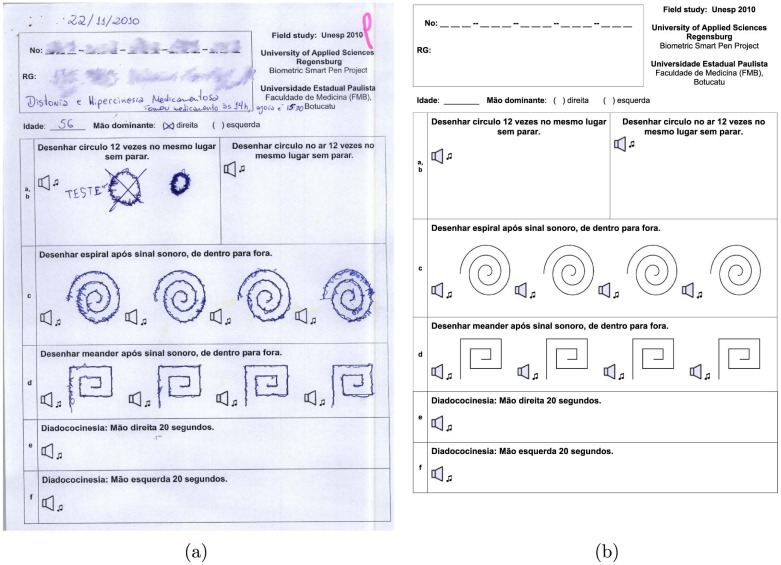
\includegraphics[width=1\textwidth]{prueba_papel}
	\caption{Prueba a papel que realizó una persona con Parkinson en este proyecto (a) y la hoja en blanco de la prueba (b).\cite{pereira2016new}}
	\label{fig:pruebapapel}
\end{figure}

A la hora de obtener el dibujo del paciente (HT), en primer lugar se filtran los dibujos para eliminar el ruido, y en el siguiente paso se utiliza una fórmula que actúe como umbral con el fin de obtener una máscara binaria \(M^{i}_{ET}\ (I)\), tal y como se muestra: 

\begin{equation}
	M^{i}_{ET}\ (I) = \left\lbrace\begin{array}{ll}
0~\text{if}R^{i}~(I)<100\wedge G^{i}~(I)<100\wedge B^{i}~(I)<100 \\ 1~\text{otherwise,} \end{array}\right.
\end{equation}

\(R^{i}(I)\), \(G^{i}(I)\) y \(B^{i}(I)\) son los valores del espacio de color RGB del píxel \(i\). Una vez obtenida la máscara \(M^{i}_{ET}\ (I)\), se restan los píxeles de la imagen original, obteniendo únicamente el dibujo del paciente.

Por otro lado, se obtiene el dibujo de la prueba (ET) de una manera similar. Se utilizan filtrados para eliminar el ruido y, a continuación, se calcula un umbral mediante una fórmula para obtener una máscara \(M^{i}_{HT}\ (F)\) que en este caso no será binaria, ya que será necesario obtener el color del bolígrafo para poder separarlo y extraer el dibujo del fondo tal y como se muestra:
 
\begin{equation}
	M^{i}_{HT}\ (F) = \left\lbrace\begin{array}{ll}
		255\begin{split}&~\text{if}|R^{i}~(F)-G^{i}~(F)|<40\wedge |R^{i}~(F)-B^{i}~(F)|<40\wedge \\ & \wedge|G^{i}-B^{i}|<40 \end{split} \\ F^i~\text{otherwise,} \end{array}\right.
\end{equation}

\(F^{i}\) es la saturación de color del píxel \(i\). Al igual que sucedía en el proceso anterior, cuando se  obtiene la máscara \(M^{i}_{HT}\ (F)\), se restan los píxeles de la imagen original, obteniendo únicamente el dibujo de la prueba.

Finalmente, se obtienen dos imágenes en cada dibujo: el dibujo del paciente y el dibujo de la prueba, como se aprecia en la figura \ref{fig:resultado}.

\begin{figure}[ht]
	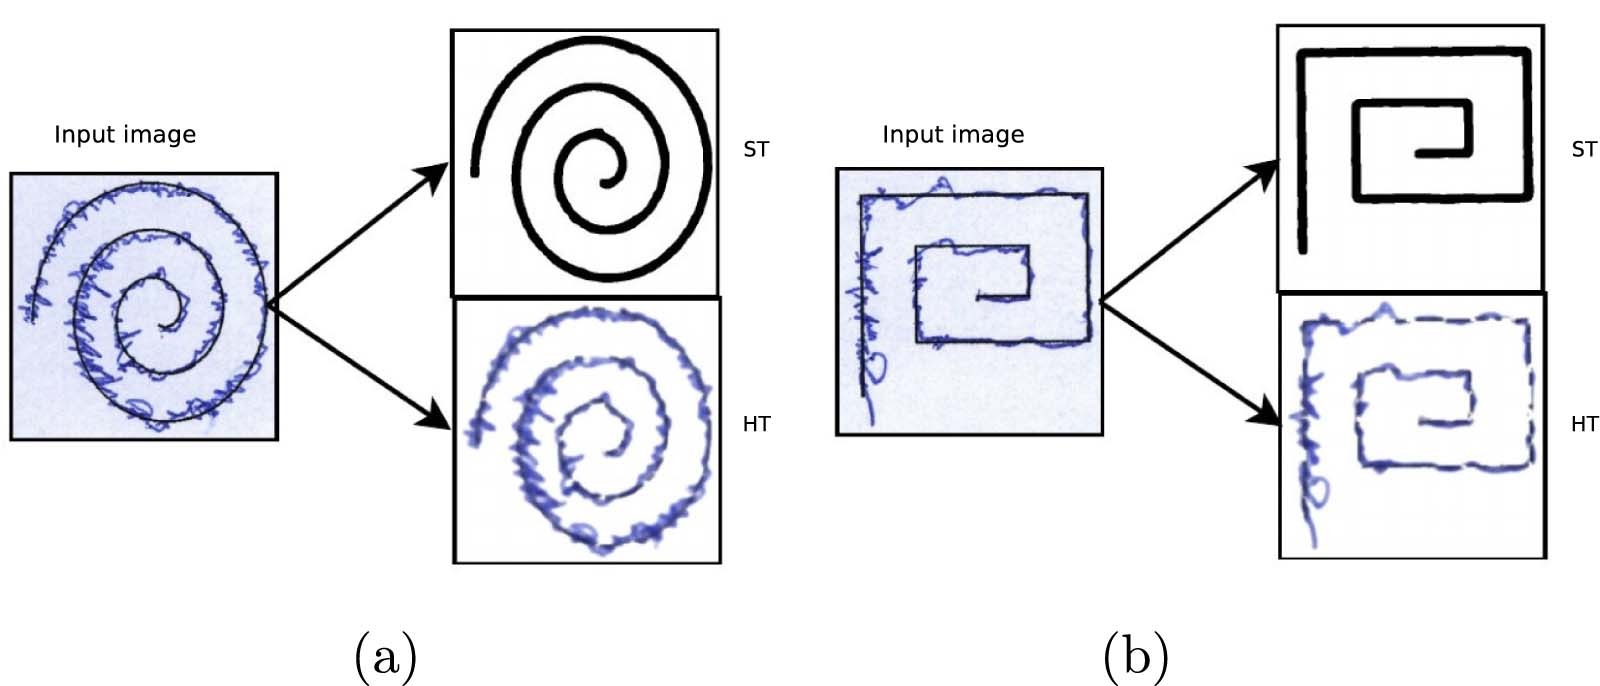
\includegraphics[width=1\textwidth]{resultado_dibujos}
	\caption{Resultado obtenido en cada dibujo del ejercicio c (a) y del ejercicio d (b).\cite{pereira2016new}}
	\label{fig:resultado}
\end{figure}

El segundo paso del proceso consiste en extraer características de los dibujos. Para ello se comparan las dos imágenes obtenidas en el primer paso para evaluar cómo de diferentes son. 

Para facilitar el proceso, se utiliza el algoritmo de adelgazamiento Zhang–Suen, que resumidamente se encarga de hacer que las trazas de los dibujos aparezcan de forma más fina. Además, se corrigen algunas imperfecciones en las imágenes, como líneas discontinuas.

Después, se enumeran algunos puntos en las imágenes y se compara la posición entre dos puntos equivalentes para conocer la desviación del dibujo del paciente con respecto al dibujo de la prueba, obteniendo varios datos con las características de los dibujos. 

También se obtienen datos obteniendo la distancia entre algunos puntos aleatorios de ambas espirales al centro, ya que la desviación del dibujo del paciente afecta también en su enfermedad de Parkinson.

Finalmente, se entrenan los modelos para detectar el Parkinson con todos los datos obtenidos en el paso anterior.

El experimento que se llevó a cabo albergaba dos grupos de personas: uno con gente sin Parkinson y otro con gente con Parkinson. Además, se mezcló en ambos grupos los dos sexos y algún zurdo, frente a una mayoría diestra.

\subsection{Proposing a Three-Stage Model to Quantify
	Bradykinesia on a Symptom Severity Level
	Using Deep Learning}
Este proyecto~\cite{jaber2021proposing} es similar al que se trata en este documento, ya que también se basa en recoger datos procesando la mano haciendo un movimiento de pinza.

Para ello, se procesan varios vídeos con la mano, tanto izquierda como derecha, habiendo además varios de control. El movimiento realizado debe ser lo más rápido y amplio posible durante 10 segundos.

El preprocesado se realiza utilizando VLC Player para obtener fotogramas de los vídeos. Con Python, y más concretamente, una biblioteca llamada LabelImg se anotan de forma gráfica objetos detectados en la imagen, como se puede observar en la figura \ref{manoetiquetada}.

\begin{figure}[]
	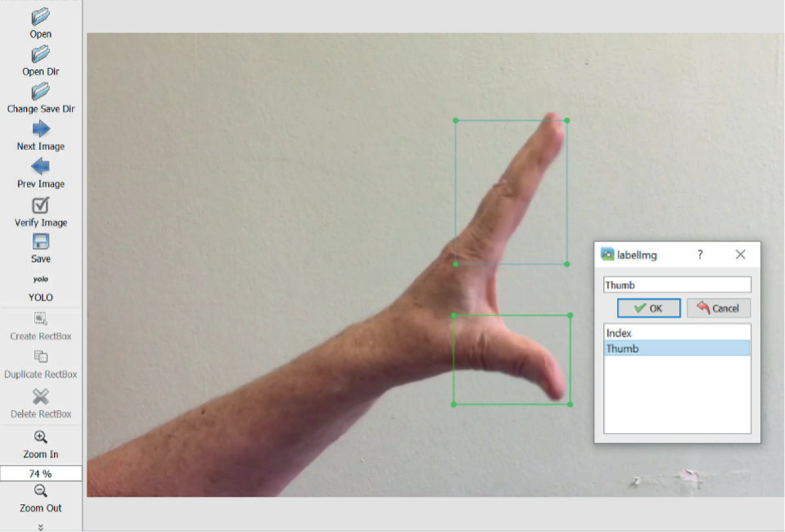
\includegraphics[width=1\textwidth]{mano_etiquetada}
	\caption{Mano con los dedos índice y pulgar etiquetados.\cite{jaber2021proposing}}
	\label{manoetiquetada}
\end{figure}

Eso servirá para recoger las coordenadas de los dedos índice y pulgar y anotarlos en un fichero de texto de la manera: 
\begin{equation}
	\text{< object - class >< x\_center >< y\_center >< width >< height >}
\end{equation}

Utilizando la herramienta YOLO, se consigue que los vídeos sean procesados en tiempo real, y así, consiguiendo más velocidad en el preprocesado.

Cada recuadro muestra el ID de la clase y la confianza de detección tal y como se ve en la figura \ref{manoetiquetas}. El movimiento se conoce comparando las coordenadas del recuadro con las coordenadas del recuadro que tenía el fotograma anterior, lo cual se almacena para cada fotograma junto al momento en el que se calcula.

\begin{figure}[]
	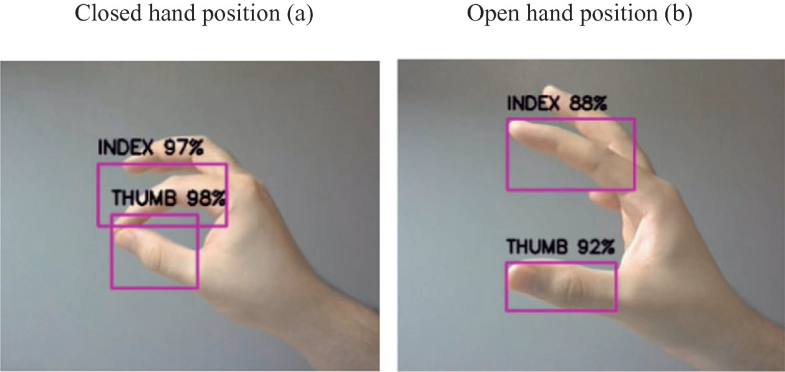
\includegraphics[width=1\textwidth]{mano_etiquetas}
	\caption{Detección realizada con un ajuste ideal.\cite{jaber2021proposing}}
	\label{manoetiquetas}
\end{figure}

En caso de haber ruido de fondo y/o una orientación de la mano diferente, podría afectar a la confianza de detección, empeorando los resultados obtenidos.

Estos datos obtenidos se utilizan para realizar cálculos con los que sacar conclusiones. Entre los cálculos se encuentran:

\begin{itemize}
	\item Separación: es el desplazamiento entre dos recuadros.
	\item Tiempo: se obtiene extrayendo el fotograma actual y restándole el anterior dividido entre los fotogramas capturados por segundo.
	\item Velocidad: se calcula con la diferencia de separación entre dos fotogramas contiguos dividido entre el tiempo.
	\item Ritmo: es el producto entre la diferencia de separación de dos fotogramas contiguos y su respectiva velocidad.
\end{itemize}

Finalmente, los datos se representan en gráficas observar las diferencias de las personas que padecen Parkinson de las que no y con ello alcanzar conclusiones.

\subsection{Tabla de medidas}
En esta sección se recoge de manera resumida en una tabla aquellas medidas que han sido utilizadas en los trabajos expuestos anteriormente.

\begin{table}[h]
	\begin{center}
		\begin{tabular}{| c | c | c | c | c | c |}
			\hline
			Trabajo & Amplitud & Tiempo & Velocidad & Ritmo & Comparación \\ \hline
			1 &  &  &  &  & X \\
			2 & X & X & X & X & \\ 
			Este trabajo & X &  &  &  & \\ \hline
		\end{tabular}
		\caption{Tabla que resume las medidas utilizadas para detectar el Parkinson.}
		\label{tab:fruta}
	\end{center}
\end{table}
